% ------------------------------------------------------------------------------------------
%     前言区域
% ------------------------------------------------------------------------------------------
\documentclass{beamer}
\usepackage{ctex, hyperref}
\usepackage[T1]{fontenc}

% other packages
\usepackage{latexsym,amsmath,xcolor,multicol,booktabs,calligra}
\usepackage{graphicx,pstricks,listings,stackengine}
\usepackage{tabularx}
\usepackage{tikz}
\usetikzlibrary{positioning, shapes.geometric}
% ------------------------------------------------------------------------------------------
%     标题页
% ------------------------------------------------------------------------------------------
\author{主讲人:吴河山}
\title{基于深度学习的井盖识别系统}
\subtitle{软件工程课程设计\newline 项目介绍与系统分析部分讲解}
\institute{计算机与信息安全学院}
\date{小组成员:刘思语\, 何冬梅}
\usepackage{GUET-Beamer}
\logo{
\includegraphics[width=2 cm]{Guet-logov.pdf}} % 每一页添加logo

% defs
\def\cmd#1{\texttt{\color{red}\footnotesize $\backslash$#1}}
\def\env#1{\texttt{\color{blue}\footnotesize #1}}
\definecolor{deepblue}{rgb}{0,0,0.5}
\definecolor{deepred}{rgb}{0.6,0,0}
\definecolor{deepgreen}{rgb}{0,0.5,0}
\definecolor{halfgray}{gray}{0.55}

\lstset{
    basicstyle=\ttfamily\small,
    keywordstyle=\bfseries\color{deepblue},
    emphstyle=\ttfamily\color{deepred},    % Custom highlighting style
    stringstyle=\color{deepgreen},
    numbers=left,
    numberstyle=\small\color{halfgray},
    rulesepcolor=\color{red!20!green!20!blue!20},
    frame=shadowbox,
}

\graphicspath{{./Picture/}} % 图片所在位置

% ------------------------------------------------------------------------------------------
%     正文
% ------------------------------------------------------------------------------------------
\begin{document}

\kaishu
\begin{frame}
    \titlepage
    \begin{figure}[htpb]
        \begin{center}
            
\includegraphics[width=0.2\linewidth]{Guet-logo.pdf}
        \end{center}
    \end{figure}
\end{frame}

\begin{frame}
    \tableofcontents[sectionstyle=show,subsectionstyle=show/shaded/hide,subsubsectionstyle=show/shaded/hide]
\end{frame}


\section{绪论}
\subsection{课题背景}
\subsubsection{社会背景}
\begin{frame}{为什么选择这个课题?}
\begin{textbox}{社会背景}
    \begin{itemize}[<+-| alert@+>] % 当然,除了alert,手动在里面插 \pause 也行
        \item 我国经济的快速发展,加快了城镇化的步伐,大小城市中用于排水等各种公共地下管线设施日益普及,道路上的井盖数量和分布也日益增多
        \item 城市里数口庞大的井盖,因为缺乏有效监控和管理,己经成为了公共安全的巨大隐患,威胁着人们的生命财产安全
        \item 井盖管理是城市文明的一部分,对于保障公共安全和提高生活质量有着重要的社会意义
    \end{itemize}
\end{textbox}
    
\end{frame}
\subsubsection{技术背景}
\begin{frame}{为什么选择这个课题?}
\begin{textbox}{技术背景}
    \begin{itemize}[<+-| alert@+>] % 当然,除了alert,手动在里面插 \pause 也行
        \item 传统的井盖检测方法已经不能满足当前的需求和挑战,需要寻找更先进和有效的方法
        \item 基于机器学习的井盖识别方法是一种有前景和优势的方法,可以克服传统方法的缺陷,提高检测的正确率和实用性
    \end{itemize}
    \end{textbox}
\end{frame}


\subsection{研究现状}

\begin{frame}{研究现状}
\begin{block}{传统方法}
	\begin{itemize}[<+-| alert@+>]
        \item 近年来,许多研究人员\cite{基于卷积神经网络的窨井盖检测,基于改进的卷积神经网络的道路井盖缺陷检测研究}都致力于道路井盖缺陷识别这一课题。然而,大多数方法都是通过硬件设计来实现
        \item 布置传感器进行检测,将检测到的数据发送到监控中心进行分析,从而实现井盖缺陷的识别
    \end{itemize}
\end{block}	
\begin{textbox}{前沿技术}
    \begin{itemize}[<+-| alert@+>]
        \item 物体识别是计算机视觉和人工智能的热门课题,有广泛的应用和价值
        \item 传统方法依赖人工特征和浅层模型,难以适应复杂场景和高精度要求
        \item 流行的深度学习方法通过神经网络自动提取特征和分类,能够适应复杂函数和环境,但仍存在网络复杂、数据量大和速度慢等问题
    \end{itemize}
    \end{textbox}
\end{frame}

\subsection{主要工作}
\begin{frame}{主要工作}
\begin{block}{项目工作}
    本项目从自动化城市管理的角度出发,设计实现在 Python 开发环境下基于深度学习的 $YOLOv3$ 算法进行井盖缺陷识别。
    \end{block}
    \begin{itemize}[<+-| alert@+>]
    \item 以树莓派为识别处理硬件,结合树莓派配置摄像头进行视觉识别
    \item 使用$YOLOv3$算法,根据训练模型,从导入的井盖图像以及知识库中学习,最终实现在测试图像中识别出井盖
    \item 系统将识别到的井盖完整度和井盖当前图像反馈到云端服务器监管平台
    \end{itemize}
\end{frame}

\section{系统分析}

\subsection{可行性分析}

\begin{frame}{技术可行性}
\begin{block}{视频与图像处理技术}
在对视频或图像进行处理的方法中,采用了形状识别和多项技术来实现井盖的标记和采集。
 \end{block}
    \begin{itemize}[<+-| alert@+>]
        \item 形状识别:该方法具有较高的识别率达到90\%。同时,该识别算法简单易懂,易于实现和应用
        \item 光线补偿技术:不同环境光下调整图像的亮度,提高图像的可辨识度
        \item 高斯平滑技术:消除噪声的干扰
        \item 灰度变换与均衡技术:使图像更加清晰、鲜明,有利于后续的识别和分析。
    \end{itemize}
\end{frame}

\subsection{操作可行性}

\begin{frame}{操作可行性}
基于深度学习的井盖识别系统运行在以下环境中:存储空间:16GB以上,内存 8G 以上。安装有 Linux 或Windows等操作系统中。另还装有摄像头进行图片采集和识别,该系统主要使用的为 CMOS 摄像头,也可使用 USB摄像头来进行图像的采集。
\newline

因此从操作可行性来看只要系统用户的硬件软件设备满足如上的要求,就可以使用该系统进行井盖的识别。
    % \begin{itemize}
    %     \item \LaTeX 广泛用于学术界,期刊会议论文模板
    % \end{itemize}
    % \begin{table}[h]
    %     \centering
    %     \begin{tabular}{c|c}
    %         Microsoft\textsuperscript{\textregistered}  Word & \LaTeX \\
    %         \hline
    %         文字处理工具 & 专业排版软件 \\
    %         容易上手,简单直观 & 容易上手 \\
    %         所见即所得 & 所见即所想,所想即所得 \\
    %         高级功能不易掌握 & 进阶难,但一般用不到 \\
    %         处理长文档需要丰富经验 & 和短文档处理基本无异 \\
    %         花费大量时间调格式 & 无需担心格式,专心作者内容 \\
    %         公式排版差强人意 & 尤其擅长公式排版 \\
    %         二进制格式,兼容性差 & 文本文件,易读、稳定 \\
    %         付费商业许可 & 自由免费使用 \\
    %     \end{tabular}
    % \end{table}
\end{frame}
\subsection{应用可行性}
\begin{frame}{应用可行性}
    \begin{minipage}{0.3\linewidth}
        \medskip
        %\hspace{2cm}
        \begin{figure}[h]
            \centering
            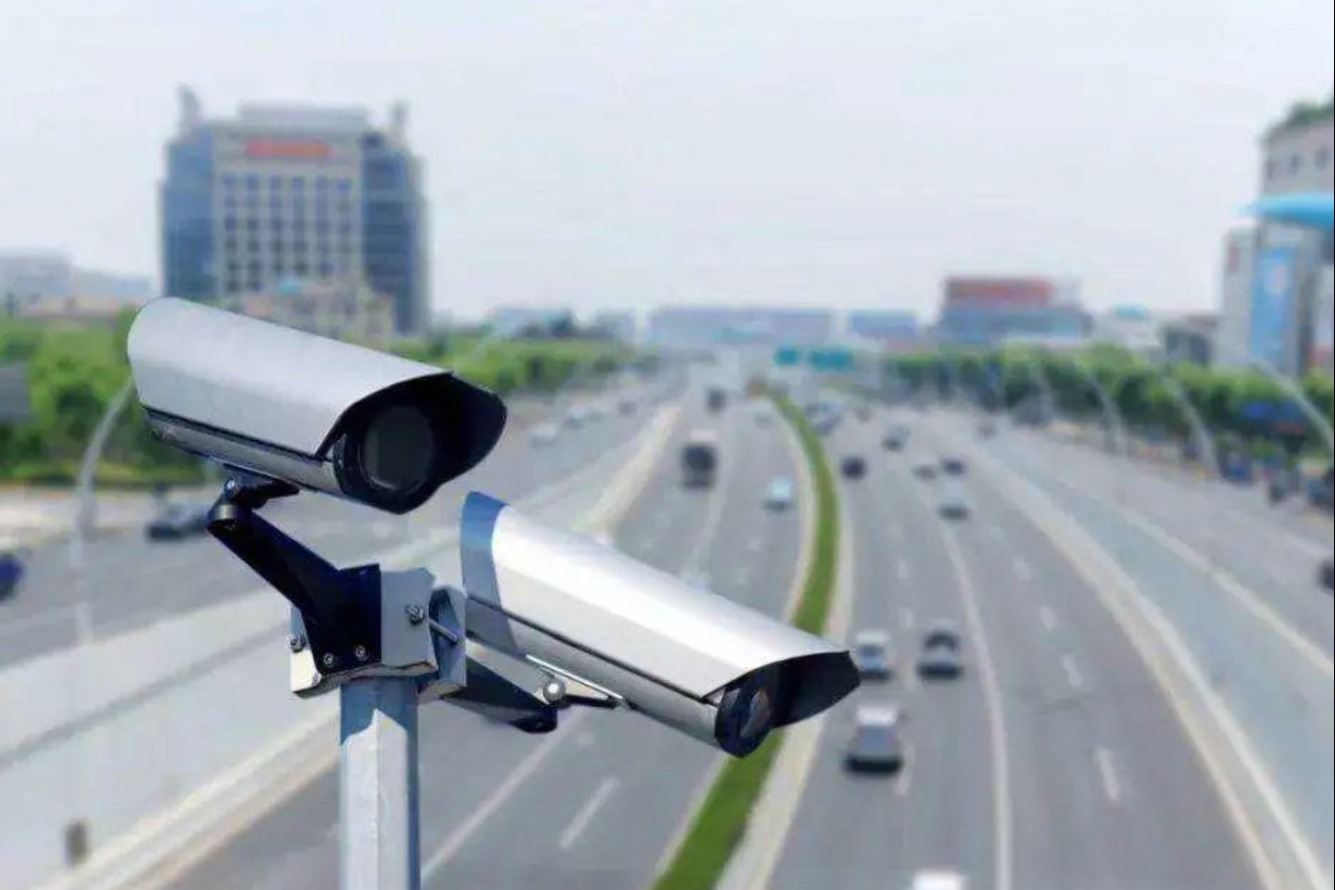
\includegraphics[height=.4\textheight]{jk.jpeg}
        \end{figure}
    \end{minipage}\hspace{2cm}
    \begin{minipage}[c]{0.5\linewidth}
只需在街道周围有井盖的地方安装摄像头,再将摄像头与系统相连,在24小时的监控下对视频文件的识别就能对井盖进行实时的监管,与监管交通的摄像头同个逻辑,无需附加过多的设备。
\end{minipage}
\end{frame}


\section{需求分析}
\subsection{用户及其功能}
\begin{frame}{用户及其功能}
该系统面向的用户是整个社会,有井盖的地方都可以使用,其功能是对井盖进行监控,当井盖发生破损,能及时向有关部门报警,以便及时安排人员去维修,减少井盖意外的发生。

 \begin{figure}[h]
            \centering
            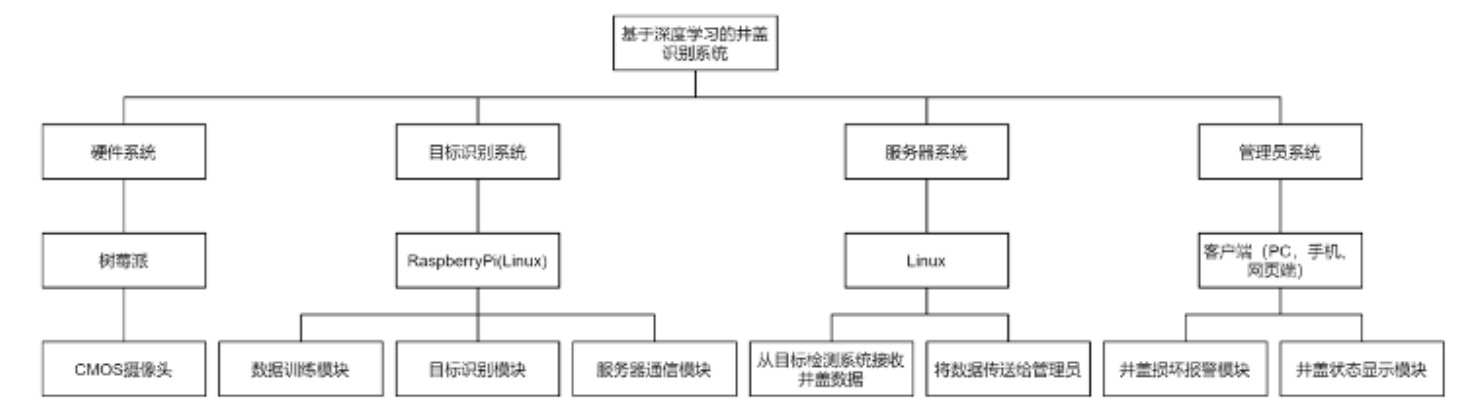
\includegraphics[height=.3\textheight]{szt.png}
            \label{层次方框图}
             \caption{层次方框图}
        \end{figure}
\end{frame}

\subsection{处理流程}
\begin{frame}{处理流程}
     \begin{figure}[h]
            \centering
            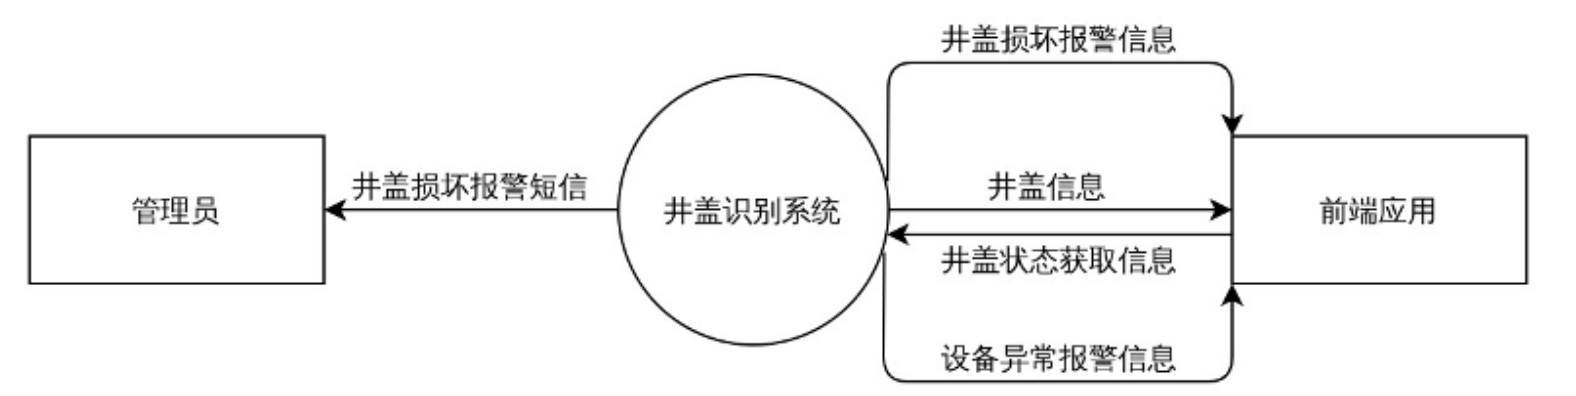
\includegraphics[height=.2\textheight]{dc.png}
            \label{顶层数据流图}
             \caption{顶层数据流图}
        \end{figure}
        \begin{figure}[h]
            \centering
            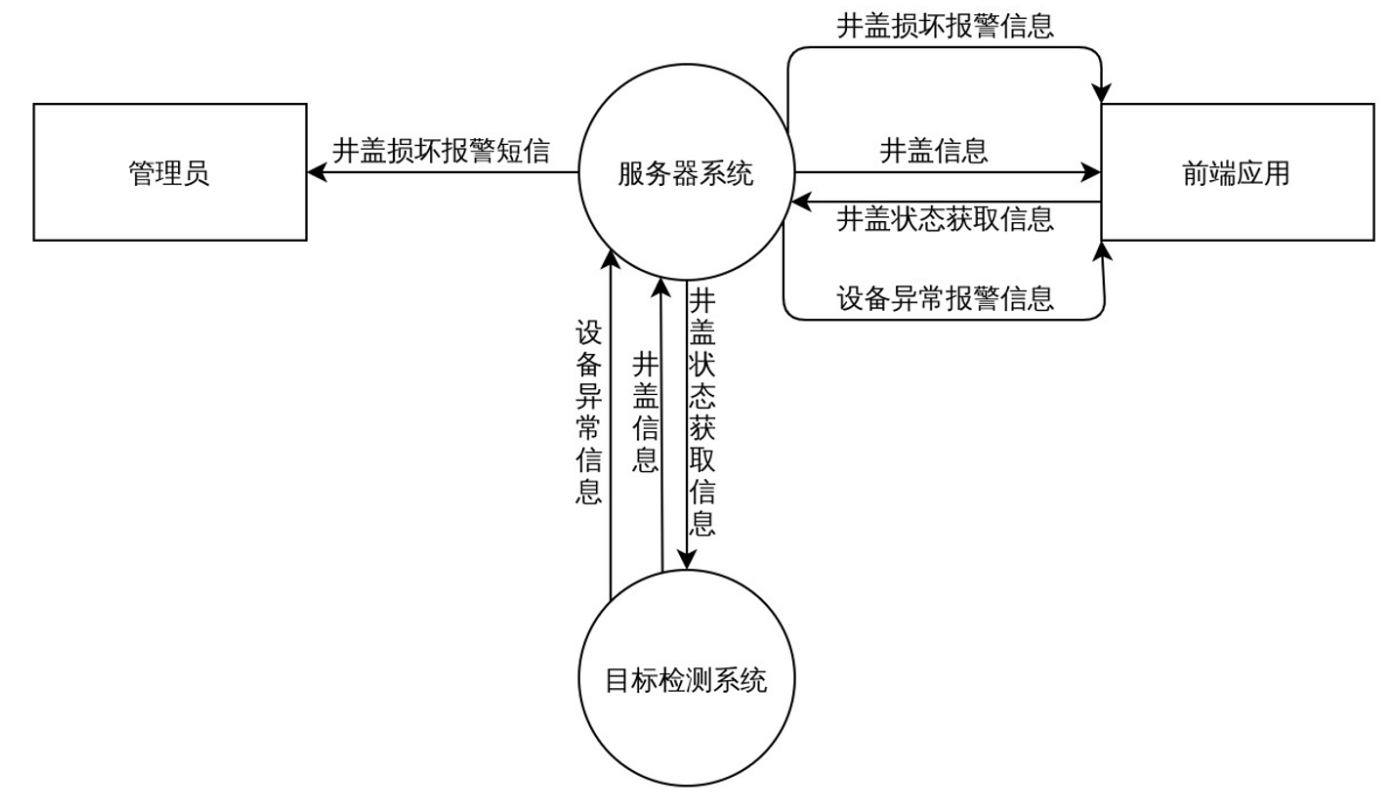
\includegraphics[height=.4\textheight]{lc.png}
            \label{零层数据流图}
             \caption{零层数据流图}
        \end{figure}
\end{frame}

\section{总体分析}
\begin{frame}{总体分析}
    \begin{minipage}{0.3\linewidth}
        \medskip
        %\hspace{2cm}
        \begin{figure}[h]
            \centering
            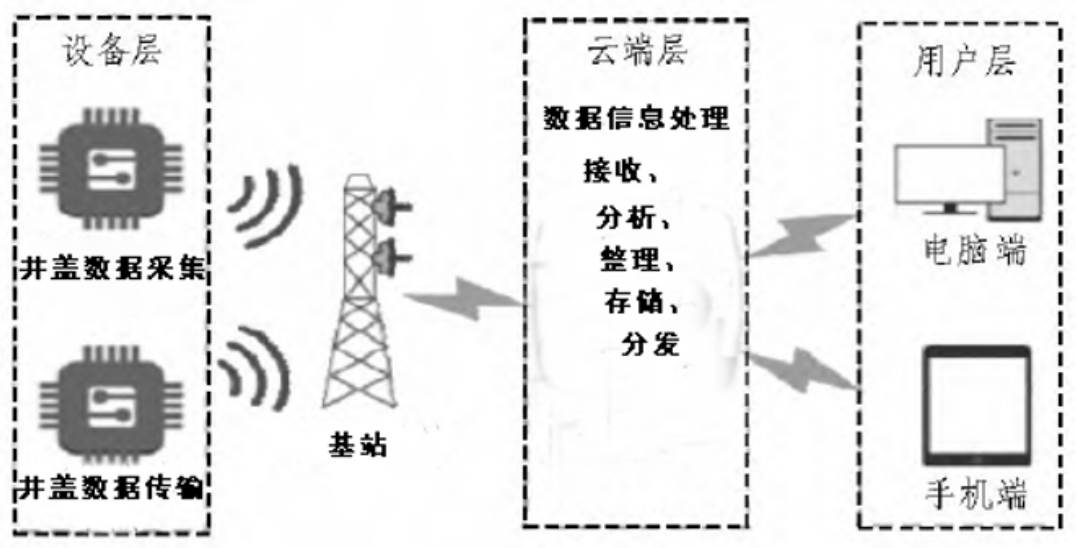
\includegraphics[height=.4\textheight]{tpt.png}
            \caption{系统拓扑图}
            \label{系统拓扑图}
        \end{figure}
    \end{minipage}\hspace{4cm}
    \begin{minipage}[c]{0.3\linewidth}
井盖识别系统分为设备层、云端层和用户层,其系统拓扑图如图\ref{系统拓扑图}所示。
\end{minipage}
\end{frame}
\subsection{系统结构图}
\begin{frame}{系统结构图}
      \begin{figure}[h]
            \centering
            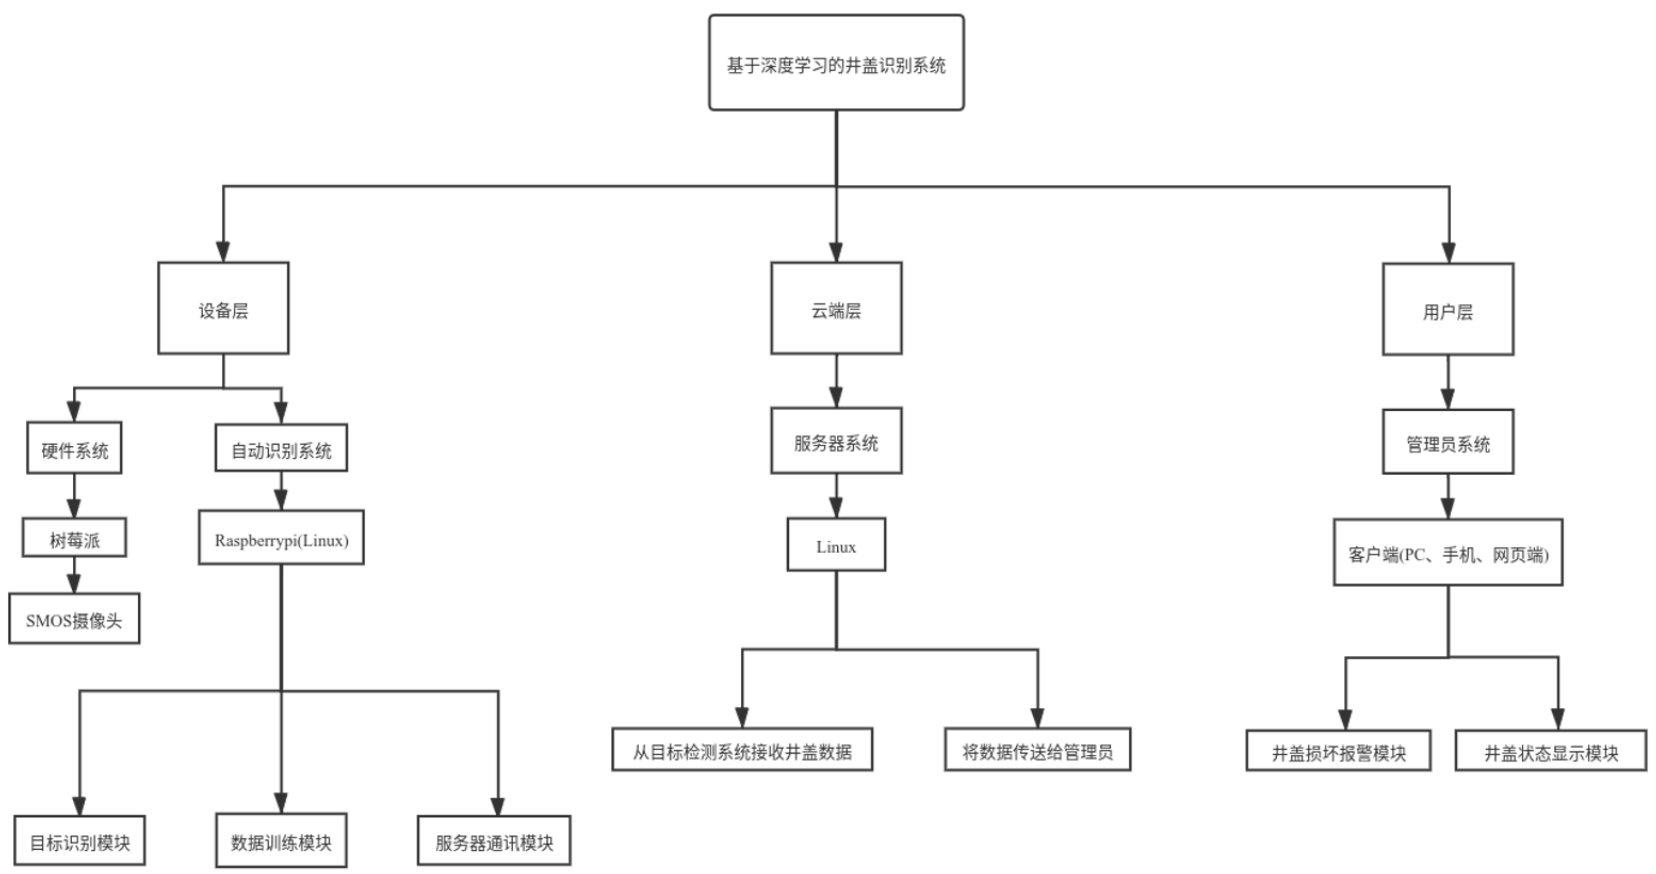
\includegraphics[height=.7\textheight]{Picture/stjg.png}
            \caption{系统结构图}
            \label{系统结构图}
        \end{figure}
\end{frame}

\subsection{设备层硬件设计}
\begin{frame}{系统设备层硬件设计}
\begin{textbox}{硬件设备}
    \begin{minipage}{0.25\linewidth}
        \medskip
        %\hspace{2cm}
        \begin{figure}[h]
            \centering
            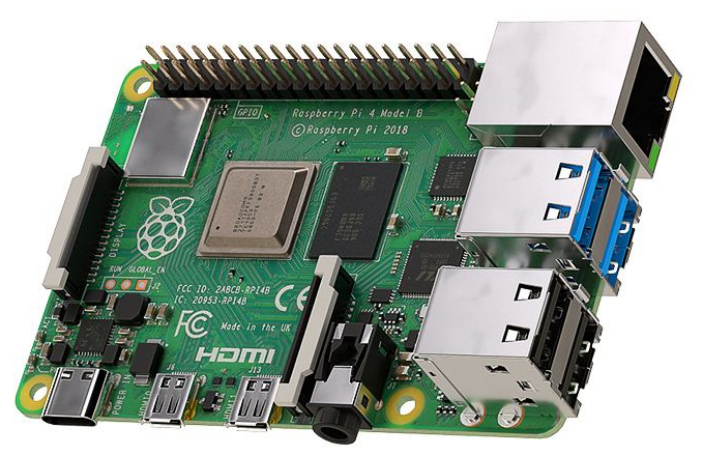
\includegraphics[height=.25\textheight]{smp.png}
            \caption{树莓派}
            \label{树莓派}
        \end{figure}
    \end{minipage}\hspace{1cm}
    \begin{minipage}{0.25\linewidth}
        \medskip
        %\hspace{2cm}
        \begin{figure}[h]
            \centering
            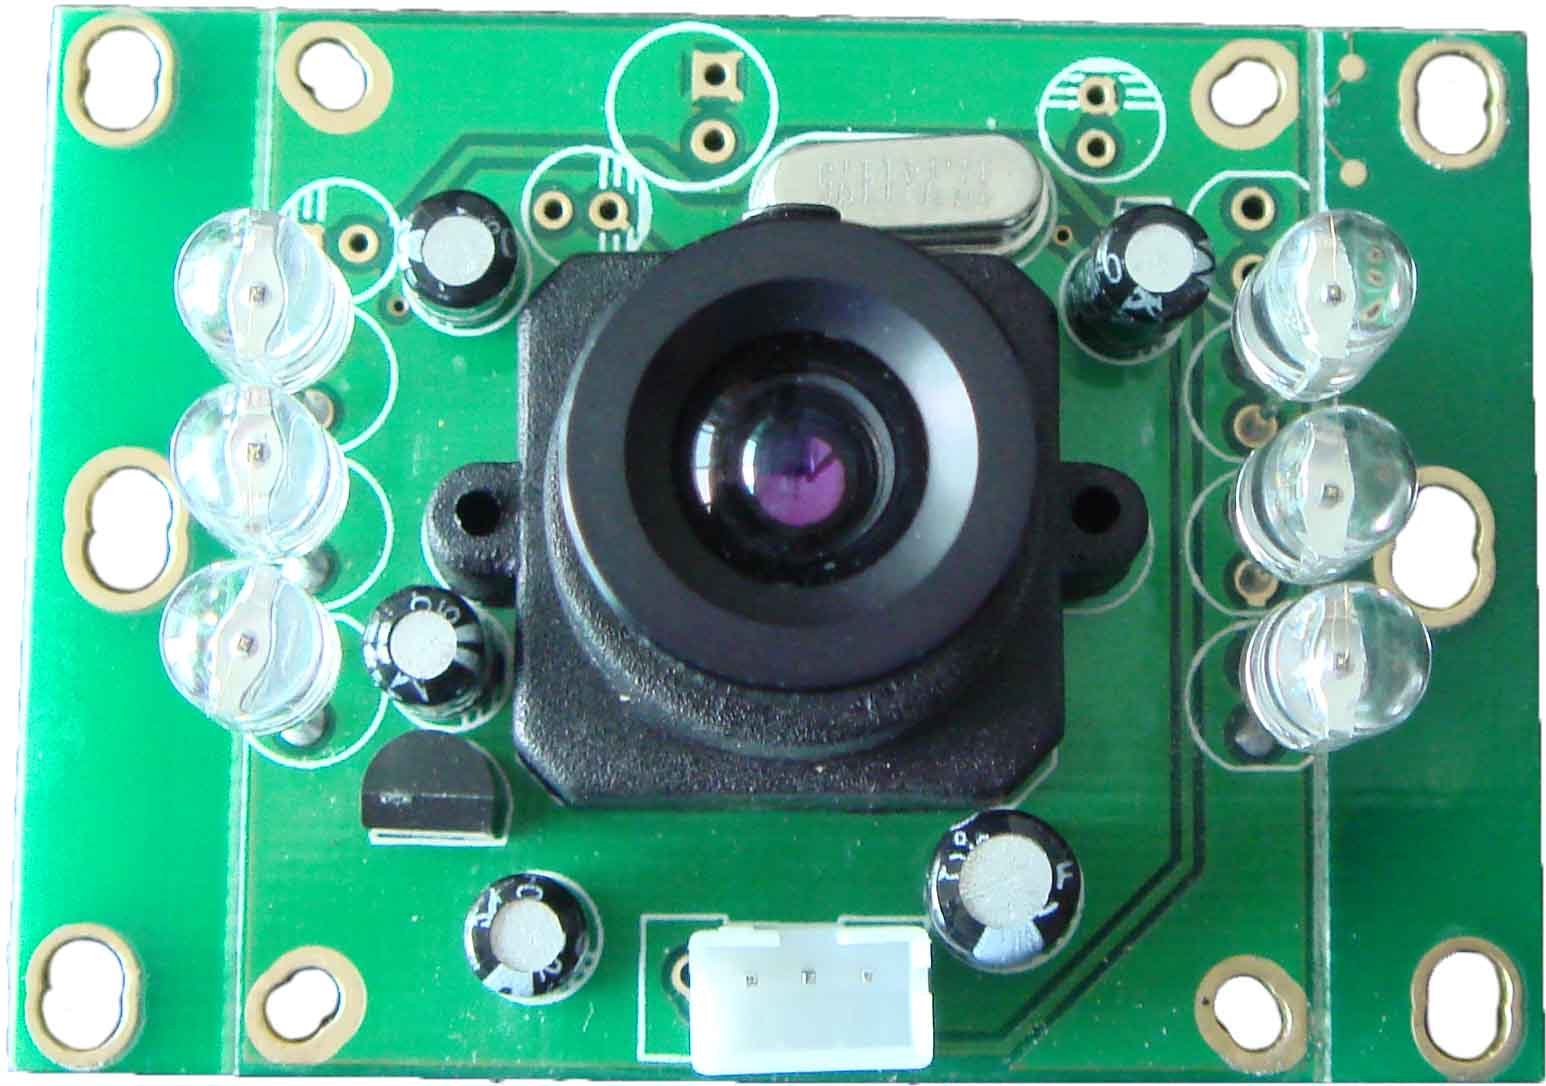
\includegraphics[height=.25\textheight]{Picture/sxt.jpeg}
            \caption{摄像头}
            \label{摄像头}
        \end{figure}
    \end{minipage}\hspace{1cm}
    \begin{minipage}{0.25\linewidth}
        \medskip
        %\hspace{2cm}
        \begin{figure}[h]
            \centering
            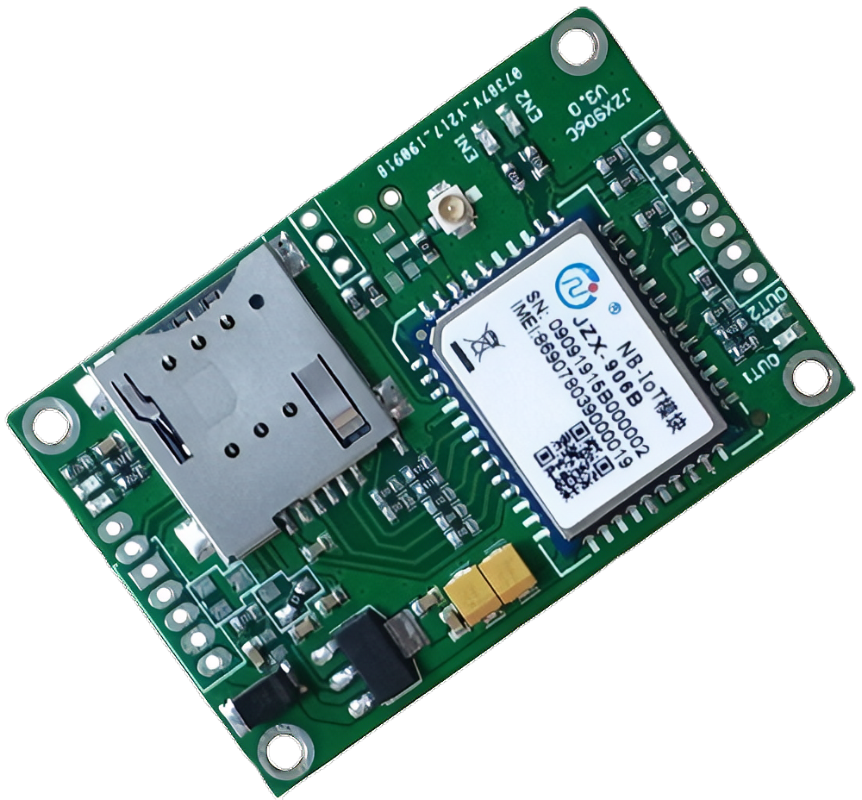
\includegraphics[height=.25\textheight]{Picture/nb.png}
            \caption{通信模块}
            \label{NB-IoT 通信模块}
        \end{figure}
    \end{minipage}
    \end{textbox}
\end{frame}

\subsection{设备层软件设计}
\begin{frame}{设备层软件设计}
    井盖识别系统设备层的软件功能主要包括模块初始化、数据采集与发送、低功耗模式和异常处理等。
    \begin{figure}[!h]
\centering
\begin{tikzpicture}[node distance=5pt]
  \node[draw, rounded corners]                        (start)   {开始};
  \node[draw, below=of start]                         (step 1)  {云端更新同步指令};
  \node[draw, below=of step 1]                        (step 2)  {模块初始化};
  \node[draw, below=of step 2]     (step 3)  {传感器采集数据};
   \node[draw, diamond, aspect=2, below=of step 3]     (choice)  {异常检测};
   \node[draw, right=30pt of choice]      (step 4)  {通知云端推送};
   \node[draw, left=40pt of choice]      (step 5)  {持续关注};
   
  \draw[->] (start)  -- (step 1);
  \draw[->] (step 1) -- (step 2);
  \draw[->] (step 2) -- (step 3);
  \draw[->] (step 3) -- (choice);
 \draw[->] (choice) -- node[above]  {异常} (step 4);
  \draw[->] (choice) -- node[above] {无异常}  (step 5);
  \draw[->] (step 5) --  (step 5|-step 3) --(step 3);
  \draw[->] (step 4) -- (step 4|-step 3) -- node[above] {解决问题}(step 3);
\end{tikzpicture}
\caption{设备层软件工作流程图}
\end{figure}
\end{frame}

\subsection{云端层设计}
\begin{frame}{系统云端层设计}
系统使用阿里物联网云平台和云服务器所组成的云端层,作为设备和用户层的中间件:
    \begin{figure}[h]
            \centering
            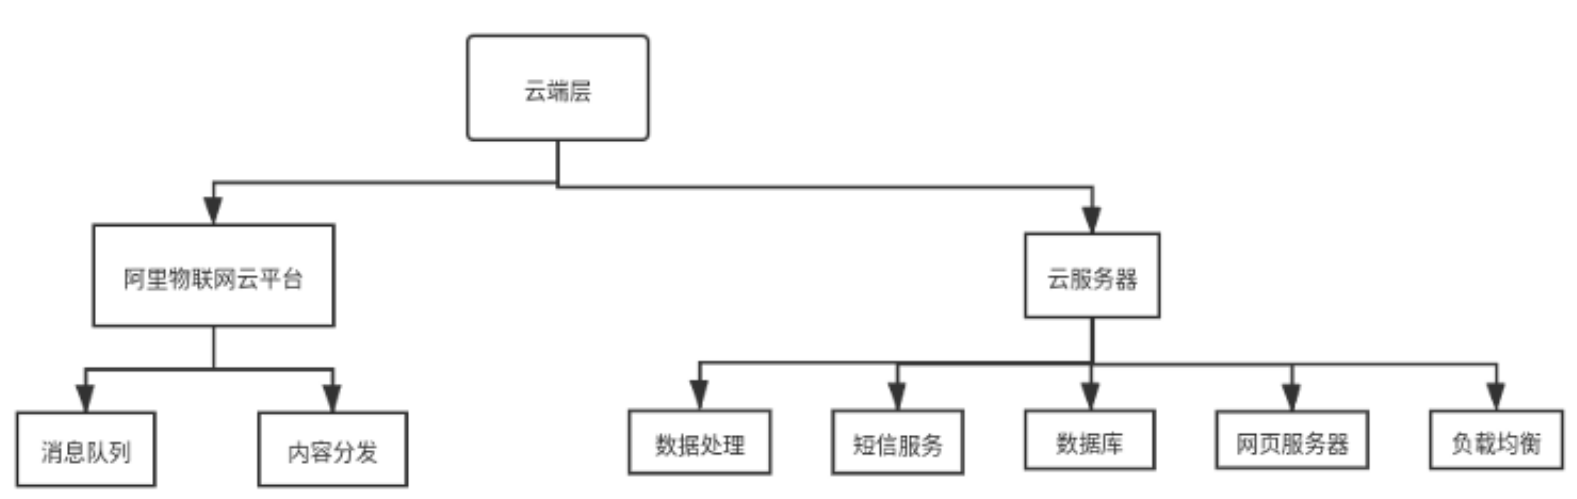
\includegraphics[height=.4\textheight]{Picture/aly.png}
            \caption{系统云端层}
            \label{系统云端层}
        \end{figure}
\end{frame}

\subsection{用户层设计}
\begin{frame}{系统用户层设计}
系统用户层通过网页来实现对用户与设备的图形化管理,前期使用Python GUI进行模拟。
    \begin{figure}[h]
            \centering
            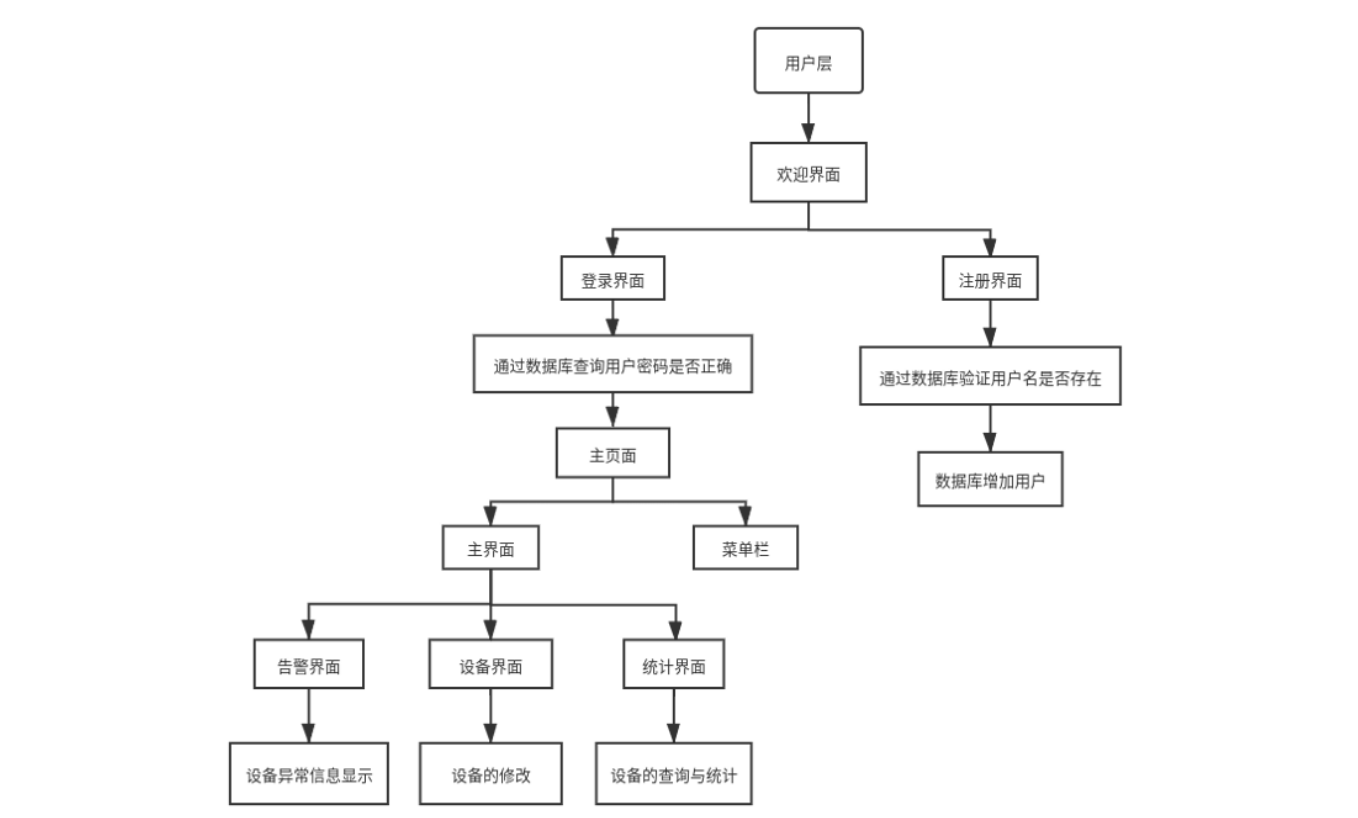
\includegraphics[height=.6\textheight]{Picture/yh.png}
            \caption{系统用户层流程图}
            \label{系统用户层流程图}
        \end{figure}
\end{frame}
% \begin{frame}{排版举例}
	
% 	\begin{textbox}{无编号公式}
%         \begin{equation*}
%             J(\theta) = \mathbb{E}_{\pi_\theta}[G_t] = \sum_{s\in\mathcal{S}} d^\pi (s)V^\pi(s)=\sum_{s\in\mathcal{S}} d^\pi(s)\sum_{a\in\mathcal{A}}\pi_\theta(a|s)Q^\pi(s,a)
%         \end{equation*}
%     \end{textbox}
%     \begin{textbox}{多行多列公式\footnotemark[1]}
%         % 使用 & 分隔
%         \begin{align}
%             Q_\mathrm{target}&=r+\gamma Q^\pi(s^\prime, \pi_\theta(s^\prime)+\epsilon)\\
%             \epsilon&\sim\mathrm{clip}(\mathcal{N}(0, \sigma), -c, c)\nonumber
%         \end{align}
%     \end{textbox}
%     \footnotetext[1]{如果公式中有文字出现,请用 $\backslash$mathrm\{\} 或者 $\backslash$text\{\} 包含,不然就会变成 $clip$,在公式里看起来比 $\mathrm{clip}$ 丑非常多。}
% \end{frame}


% \begin{frame}{如何使用块}
% \begin{block}{块的名称}
% 	\begin{itemize}
%         \item A
%         \item B
%     \end{itemize}
% \end{block}	
% \end{frame}

% \begin{frame}{如何使用定义、定理、引理、证明}

% \kaishu
% \begin{define}[定义名称]
% 	定义内容
% \end{define}

% \begin{lem}[引理名称]
% 	引理内容
% \end{lem}

% \begin{thm}[定理名称]
% 	定理内容(这里的定义、引理、定理分章节自动标号)
% \end{thm}

% \begin{proof}
% 	证明内容
% \end{proof}

% \end{frame}

% \begin{frame}
%     \begin{textbox}{编号多行公式}
%         % Taken from Mathmode.tex
%         \begin{multline}
%             A=\lim_{n\rightarrow\infty}\Delta x\left(a^{2}+\left(a^{2}+2a\Delta x+\left(\Delta x\right)^{2}\right)\right.\label{eq:reset}\\
%             +\left(a^{2}+2\cdot2a\Delta x+2^{2}\left(\Delta x\right)^{2}\right)\\
%             +\left(a^{2}+2\cdot3a\Delta x+3^{2}\left(\Delta x\right)^{2}\right)\\
%             +\ldots\\
%             \left.+\left(a^{2}+2\cdot(n-1)a\Delta x+(n-1)^{2}\left(\Delta x\right)^{2}\right)\right)\\
%             =\frac{1}{3}\left(b^{3}-a^{3}\right)
%         \end{multline}
%     \end{textbox}
% \end{frame}

% \begin{frame}{图形与分栏}
%     % From thuthesis user guide.
%     \begin{minipage}[c]{0.3\linewidth}
%         \psset{unit=0.8cm}
%         \begin{pspicture}(-1.75,-3)(3.25,4)
%             \psline[linewidth=0.25pt](0,0)(0,4)
%             \rput[tl]{0}(0.2,2){$\vec e_z$}
%             \rput[tr]{0}(-0.9,1.4){$\vec e$}
%             \rput[tl]{0}(2.8,-1.1){$\vec C_{ptm{ext}}$}
%             \rput[br]{0}(-0.3,2.1){$\theta$}
%             \rput{25}(0,0){%
%             \psframe[fillstyle=solid,fillcolor=lightgray,linewidth=.8pt](-0.1,-3.2)(0.1,0)}
%             \rput{25}(0,0){%
%             \psellipse[fillstyle=solid,fillcolor=yellow,linewidth=3pt](0,0)(1.5,0.5)}
%             \rput{25}(0,0){%
%             \psframe[fillstyle=solid,fillcolor=lightgray,linewidth=.8pt](-0.1,0)(0.1,3.2)}
%             \rput{25}(0,0){\psline[linecolor=red,linewidth=1.5pt]{->}(0,0)(0.,2)}
% %           \psRotation{0}(0,3.5){$\dot\phi$}
% %           \psRotation{25}(-1.2,2.6){$\dot\psi$}
%             \psline[linecolor=red,linewidth=1.25pt]{->}(0,0)(0,2)
%             \psline[linecolor=red,linewidth=1.25pt]{->}(0,0)(3,-1)
%             \psline[linecolor=red,linewidth=1.25pt]{->}(0,0)(2.85,-0.95)
%             \psarc{->}{2.1}{90}{112.5}
%             \rput[bl](.1,.01){C}
%         \end{pspicture}
%     \end{minipage}\hspace{1cm}
%     \begin{minipage}{0.5\linewidth}
%         \medskip
%         %\hspace{2cm}
%         \begin{figure}[h]
%             \centering
%             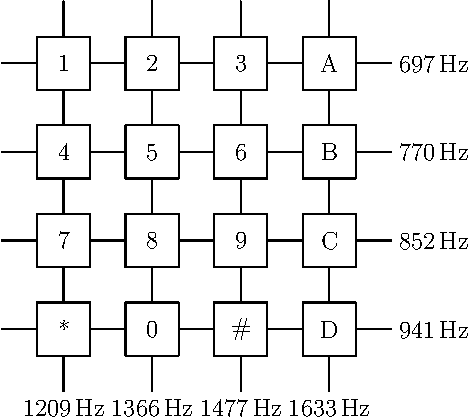
\includegraphics[height=.4\textheight]{dtmf.pdf}
%         \end{figure}
%     \end{minipage}
% \end{frame}


\section{参考文献}

\begin{frame}[allowframebreaks]
    \bibliography{ref}
    \bibliographystyle{alpha}
    % 如果参考文献太多的话,可以像下面这样调整字体:
    % \tiny\bibliographystyle{alpha}
\end{frame}

\begin{frame}
    \begin{center}
        {\Huge\calligra Thanks!}
    \end{center}
\end{frame}

\end{document}